% Sets page margins to 1", which is the academic standard
% allows the included extensions of graphic files
% sets graphic path, does not currently work because of space in folder name
% I do not remember what this does
% allows the xhead parameters (text on the top right/left areas of pages)
% \setcounter{tocdepth}{the number of depth}
% INCLUDEGRAPHICS EXPLANATION
% \includegraphics[scale=1]{name of file}
% sometimes you want to twice encase the filename in squiggly brackets. I do not know why but sometimes it is required.


\documentclass{article}
%%%%%%%%%%%%%%%%%%%%%%%%%%%%%%%%%%%%%%%%%%%%%%%%%%%%%%%%%%%%%%%%%%%%%%%%%%%%%%%%%%%%%%%%%%%%%%%%%%%%%%%%%%%%%%%%%%%%%%%%%%%%%%%%%%%%%%%%%%%%%%%%%%%%%%%%%%%%%%%%%%%%%%%%%%%%%%%%%%%%%%%%%%%%%%%%%%%%%%%%%%%%%%%%%%%%%%%%%%%%%%%%%%%%%%%%%%%%%%%%%%%%%%%%%%%%
\usepackage{geometry}
\usepackage{fancyhdr}
\usepackage[pdftex]{graphicx}

%TCIDATA{OutputFilter=LATEX.DLL}
%TCIDATA{Version=5.50.0.2953}
%TCIDATA{<META NAME="SaveForMode" CONTENT="1">}
%TCIDATA{BibliographyScheme=Manual}
%TCIDATA{Created=Monday, January 30, 2012 17:20:46}
%TCIDATA{LastRevised=Wednesday, April 18, 2012 15:55:32}
%TCIDATA{<META NAME="GraphicsSave" CONTENT="32">}
%TCIDATA{<META NAME="DocumentShell" CONTENT="Standard LaTeX\Blank - Standard LaTeX Article">}
%TCIDATA{CSTFile=40 LaTeX article.cst}

\newtheorem{theorem}{Theorem}
\newtheorem{acknowledgement}[theorem]{Acknowledgement}
\newtheorem{algorithm}[theorem]{Algorithm}
\newtheorem{axiom}[theorem]{Axiom}
\newtheorem{case}[theorem]{Case}
\newtheorem{claim}[theorem]{Claim}
\newtheorem{conclusion}[theorem]{Conclusion}
\newtheorem{condition}[theorem]{Condition}
\newtheorem{conjecture}[theorem]{Conjecture}
\newtheorem{corollary}[theorem]{Corollary}
\newtheorem{criterion}[theorem]{Criterion}
\newtheorem{definition}[theorem]{Definition}
\newtheorem{example}[theorem]{Example}
\newtheorem{exercise}[theorem]{Exercise}
\newtheorem{lemma}[theorem]{Lemma}
\newtheorem{notation}[theorem]{Notation}
\newtheorem{problem}[theorem]{Problem}
\newtheorem{proposition}[theorem]{Proposition}
\newtheorem{remark}[theorem]{Remark}
\newtheorem{solution}[theorem]{Solution}
\newtheorem{summary}[theorem]{Summary}
\newenvironment{proof}[1][Proof]{\noindent\textbf{#1.} }{\ \rule{0.5em}{0.5em}}
\geometry{left=1in,right=1in,top=1in,bottom=1in} 
\DeclareGraphicsExtensions{.pdf,.png,.jpg}
\graphicspath{{C:/Users/Odd/git/Gruppe34/FellesDoc/Ktn/KTN2/}}
\setlength{\headheight}{15.2pt}
\pagestyle{fancy}
\lhead{Gruppe 34}
\rhead{FP: KTN2}
\input{tcilatex}
\setcounter{secnumdepth}{-1}

\begin{document}


% begin title page, use \\ for newline
\begin{titlepage}
\title{Collaboration Project\\
\textbf{KTN2}\\
Gruppe 34}
% now one can list the authors, \textbf{} makes bold text
\author{Bj\o rn \AA ge Tungesvik\and Tina Syversen\and Andr\'e Philipp\and Odd Magnus Trondrud\and Eivind Kvissel\and H\aa vard H\o iby}
\maketitle
\end{titlepage}\newpage % \tableofcontents

\newpage

\section{Changes}

We increased the amount of packets in the test runs from 10 to 100.

The ServerClose and ClientClose diagrams have been updated to reflect the
fact that we used the simplySendPacket(packet) method instead of the
sendDataPacketWithRetransmission(packet) for internal packets.

The new diagrams are included below.

\subsection{ServerClose}

\includegraphics[scale=1]{ktnServerClose.png}

\subsection{ClientClose}

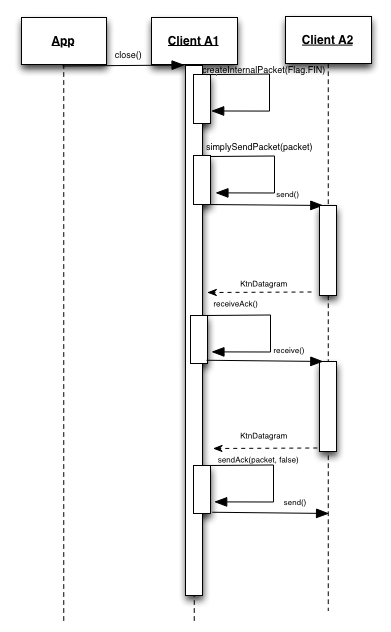
\includegraphics[scale=1]{ktnClientClose.png}

\section{Test Results}

\subsection{Initial Connection:\ T-KTN01}

\subsubsection{Result}

Three-way handshake observed. Connection successfully established.

\subsection{Connection and Tear Down:\ T-KTN02}

\subsubsection{Result}

Connection successfully established and closed. Four-way handshake observed
succeeded by a thirty second timeout on the client-side.

\section{Send and Receive:\ T-KTN03}

\subsubsection{Result}

All ten packages were received by the server.

\section{Lossy S\&R:\ T-KTN04}

\subsubsection{Result}

All 100 messages were received at both levels of error.

\section{Delayed S\&R:\ T-KTN05}

\subsubsection{Result}

All 100 messages were received at both levels of error.

\section{Lossy Delays:\ T-KTN06}

\subsubsection{Result}

All 100 messages were received at both levels of error.

\section{I ain't afraid of no ghosts:\ T-KTN07}

\subsubsection{Result}

All 100 messages were received at both levels of error.

\section{Lost Ghosts of Delay-Bay:\ T-KTN08}

\subsubsection{Result}

All 100 messages were received at both levels of error.

\section{Payload Bit Errors:\ T-KTN09}

\subsubsection{Result}

All 100 messages were received at both levels of error.

\section{Ghosts Lost in Bit Error Delays:\ T-KTN10}

\subsubsection{Result}

All 100 messages were received at both levels of error.

\section{Headless:\ T-KTN11}

\subsubsection{Result}

All 100 messages were received at both levels of error.

\section{The Full Monty:\ T-KTN12}

\subsubsection{Result}

All 100 messages were received at both levels of error.

\end{document}
